\chapter{Multimodal LLMs}

\section{Fundamentals of Multimodal Large Language Models}
Multimodal Large Language Models (MLLMs) extend traditional LLMs by incorporating multiple data modalities, such as text, images, audio, and video, enabling more comprehensive reasoning and interaction with diverse data sources.

\section*{Fine-Tuning a Transformer Model for Coastal Weather Forecasting}

{\bf Introduction}

Our introductory example describes the implementation of a fine-tuned Transformer model for processing wind field data over the North Sea. The model is based on a pretrained T5 architecture and is adapted to generate textual descriptions of wind conditions from numerical wind field inputs. The main components include synthetic wind field generation, visualization, dataset creation, model training, and evaluation.

{\bf Device Setup and Dependencies}

The implementation begins with setting up the necessary libraries, including {\tt torch} for deep learning, {\tt transformers} for handling the T5 model, and {\tt cartopy} for geospatial visualization. The computation is performed on a \emph{CUDA} device if available:

\begin{codeonly}{Device Setup}
import torch

device = torch.device("cuda" if torch.cuda.is_available() else "cpu")
print(device)
\end{codeonly}

{\bf Generating Synthetic Wind Fields}

Wind field data is generated using a grid-based approach. A base wind direction is selected, and random variations of \(\pm10\) degrees are applied at each grid point to simulate realistic wind fluctuations. The wind speed follows a controlled distribution:

\begin{codeonly}{Generate Synthetic Wind Fields}
def generate_wind_field(grid_size=10, base_wind_dir=315, wind_speed=None):
    lon = np.linspace(5, 10, grid_size)
    lat = np.linspace(53, 56, grid_size)
    LON, LAT = np.meshgrid(lon, lat)
    
    theta_variation = np.random.uniform(-10, 10, size=(grid_size, grid_size))
    theta = np.deg2rad(270 - (base_wind_dir + theta_variation))
    
    U = wind_speed * np.cos(theta)
    V = wind_speed * np.sin(theta)
    
    return LON, LAT, U, V, wind_speed
\end{codeonly}

\begin{figure}[h]
    \centering
    \begin{tabular}{cc}
        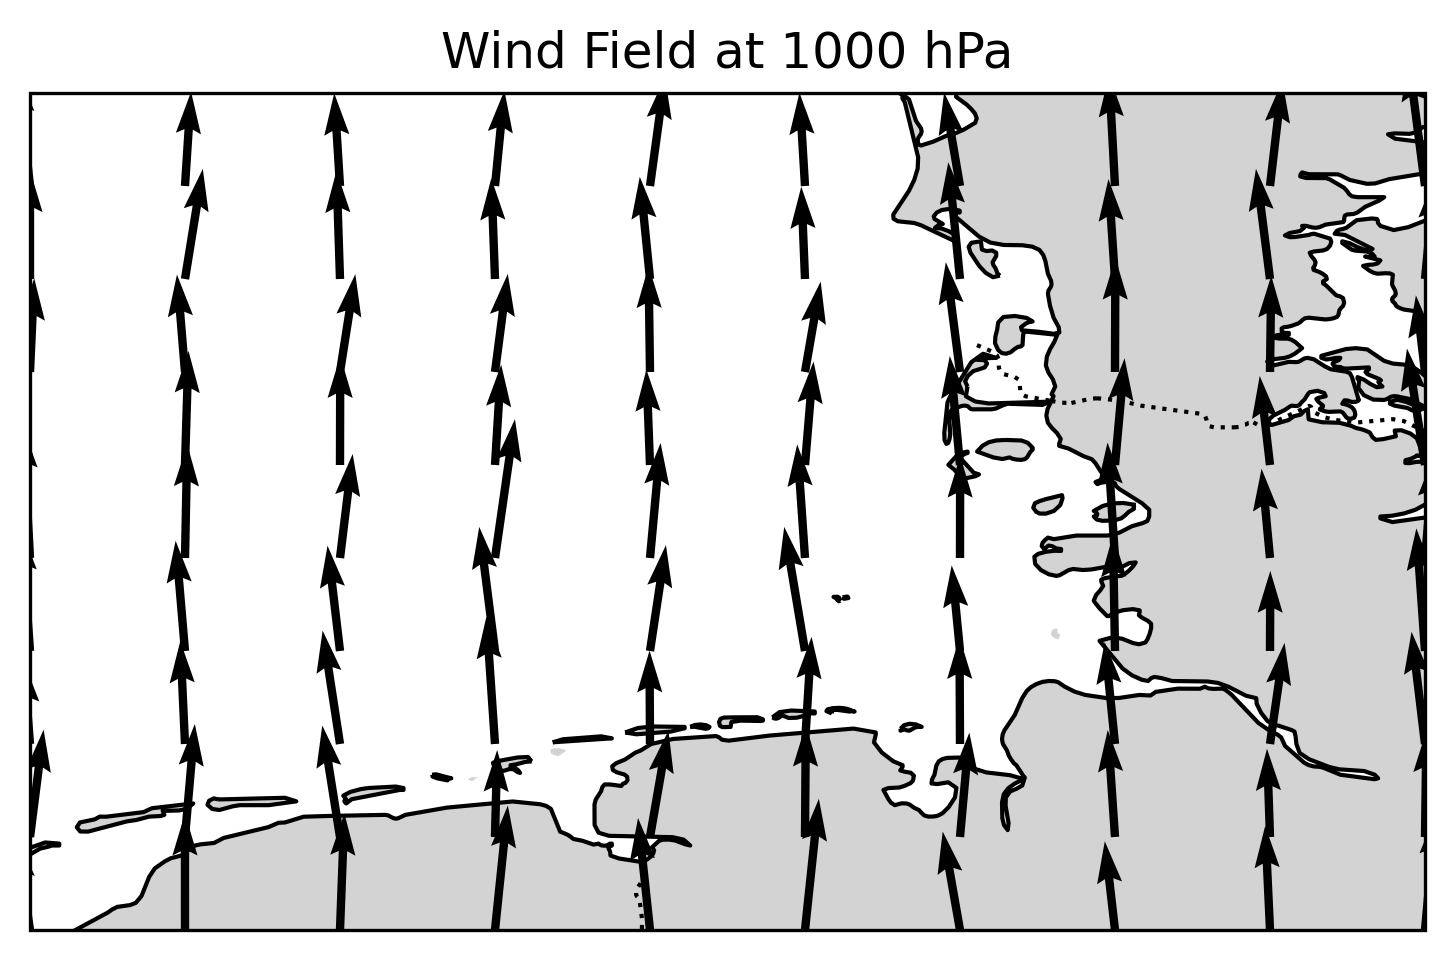
\includegraphics[width=0.6\textwidth]{images/coastal_wind.png} & 
    \end{tabular}. 
    \caption{Coastal Wind with example text description: "Strong northerly winds with speeds around 15.0 m/s over the North Sea".
}
    \label{fig:coastal_wind}
\end{figure}

{\bf Visualizing Wind Fields}

Wind fields are displayed using {\tt Cartopy}, showing vectors representing wind direction and magnitude. The following function renders the wind data on a map projection:

\begin{codeonly}{Plot Wind Fields}
def plot_wind_field(LON, LAT, U, V, title="Wind Field at 1000 hPa"):
    fig, ax = plt.subplots(figsize=(6, 4),\ 
		subplot_kw={'projection': ccrs.PlateCarree()})
    ax.set_extent([5, 10, 53, 56], crs=ccrs.PlateCarree())
    ax.add_feature(cfeature.COASTLINE)
    ax.add_feature(cfeature.BORDERS, linestyle=':')
    ax.add_feature(cfeature.LAND, facecolor='lightgray')
    ax.quiver(LON, LAT, U, V, scale=200, transform=ccrs.PlateCarree())
    ax.set_title(title)
    plt.show()
\end{codeonly}

{\bf Generating Textual Descriptions}

The model converts wind field data into descriptive text by categorizing wind intensity and associating wind direction with predefined labels. Wind speed values are rounded to predefined levels:

\begin{codeonly}{Generate Text Descriptions}
def generate_text_description(wind_speed, wind_dir):
    intensity = "strong" if np.mean(wind_speed) > 12 else "moderate" if np.mean(wind_speed) > 6 else "light"
    directions = {0: "northerly", 45: "northeasterly", 90: "easterly", 135: "southeasterly",
                  180: "southerly", 225: "southwesterly", 270: "westerly", 315: "northwesterly"}
    direction = directions.get(round(wind_dir), "variable")
    approx_speed = [0, 1, 2, 5, 10, 15, 20, 25, 30][np.argmin(np.abs([0, 1, 2, 5, 10, 15, 20, 25, 30] - np.mean(wind_speed)))]
    return f"{intensity.capitalize()} {direction} winds with speeds around {approx_speed} m/s over the North Sea."
\end{codeonly}

{\bf Training the Transformer Model}

The fine-tuning process uses a pretrained \emph{T5-small} model. Wind fields are encoded as structured text, and corresponding descriptions are used as target outputs. The model is trained using an Adam optimizer with a learning rate of \(5 \times 10^{-5}\):

\begin{codeonly}{Train Transformer Model}
def train_transformer(text_samples, wind_fields, num_epochs=10):
    tokenizer = T5Tokenizer.from_pretrained("t5-small")
    model = T5ForConditionalGeneration.from_pretrained("t5-small").to(device)
    optimizer = torch.optim.AdamW(model.parameters(), lr=5e-5)
    
    loss_history = []
    start_time = time.time()

    for epoch in range(num_epochs):
        epoch_start = time.time()
        total_loss = 0
        
        for wind, text in zip(wind_fields, text_samples):
            U, V, wind_speed = wind
            wind_input = f"Wind field: U: {' '.join(map(str, np.round(U.flatten()[:20], 2)))}; V: {' '.join(map(str, np.round(V.flatten()[:20], 2)))}; Speed: {' '.join(map(str, np.round(wind_speed.flatten()[:20], 2)))}."
            input_ids = tokenizer.encode(wind_input, return_tensors="pt", truncation=True, max_length=512).to(device)
            labels = tokenizer.encode(text, return_tensors="pt", truncation=True, max_length=512).to(device)
            outputs = model(input_ids=input_ids, labels=labels)
            loss = outputs.loss
            optimizer.zero_grad()
            loss.backward()
            optimizer.step()
            total_loss += loss.item()
        
        avg_loss = total_loss / len(text_samples)
        loss_history.append(avg_loss)
        print(f"Epoch {epoch+1}/{num_epochs} | Loss: {avg_loss:.4f}")
    
    return model, tokenizer, loss_history
\end{codeonly}

\begin{figure}[h]
    \centering
    \begin{tabular}{cc}
        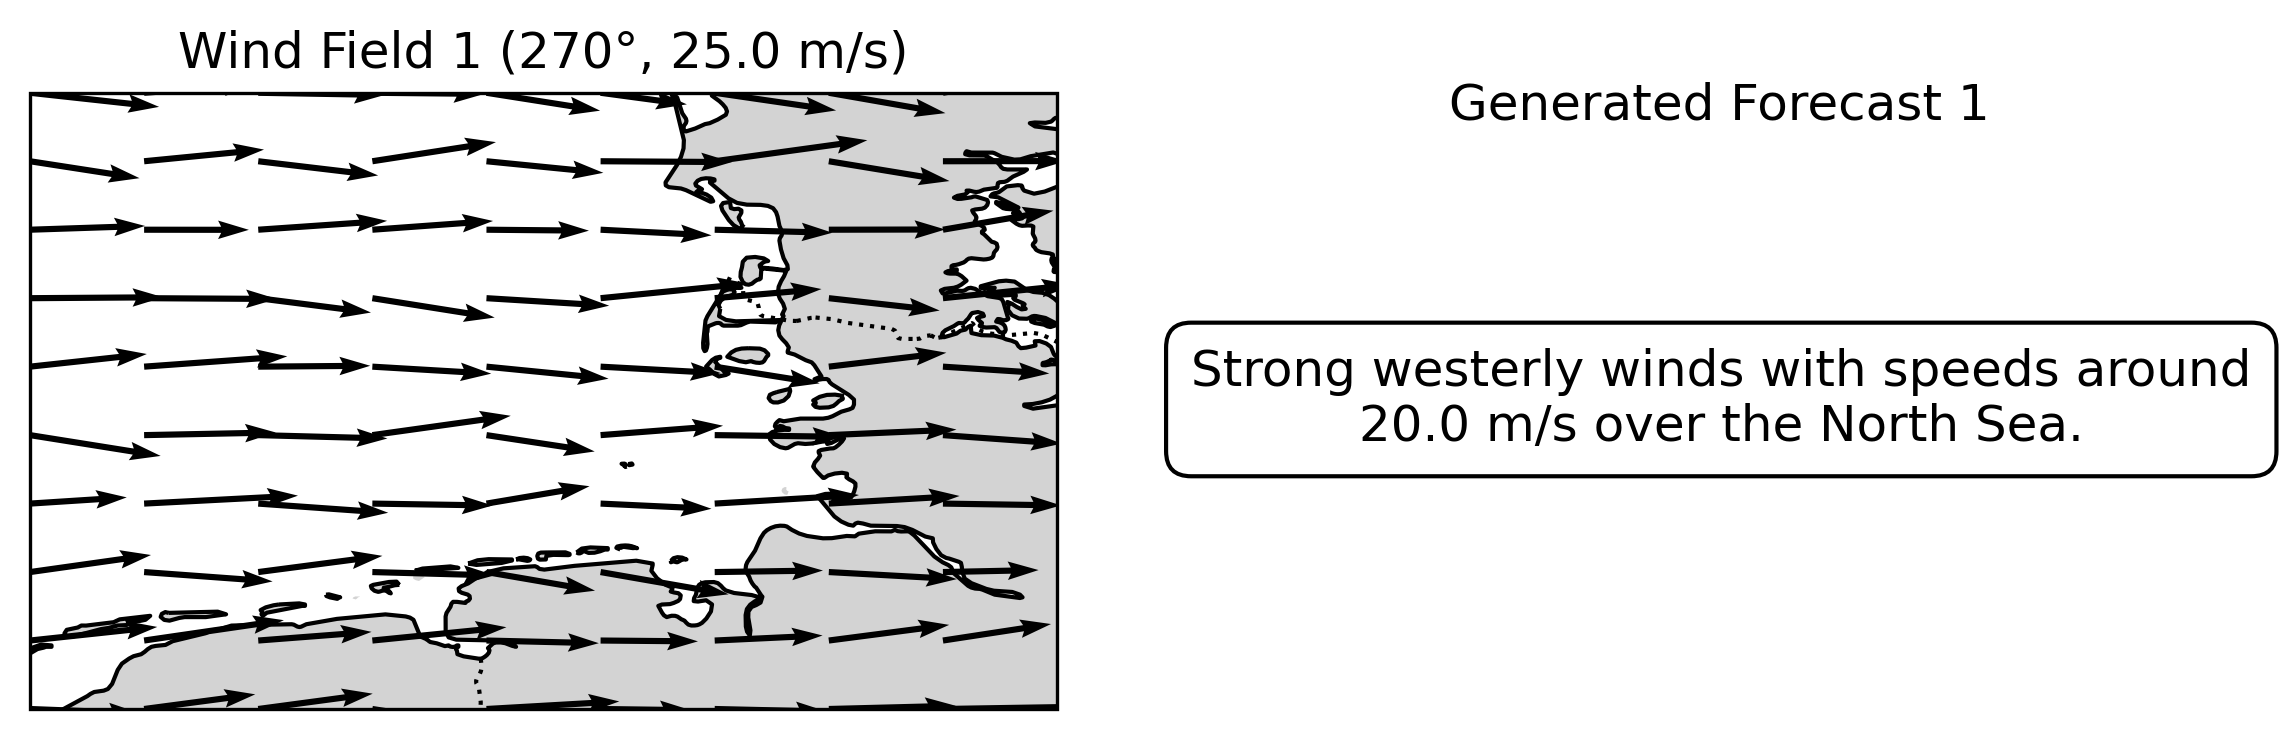
\includegraphics[width=0.45\textwidth]{images/coastal_fcst_00.png} & 
        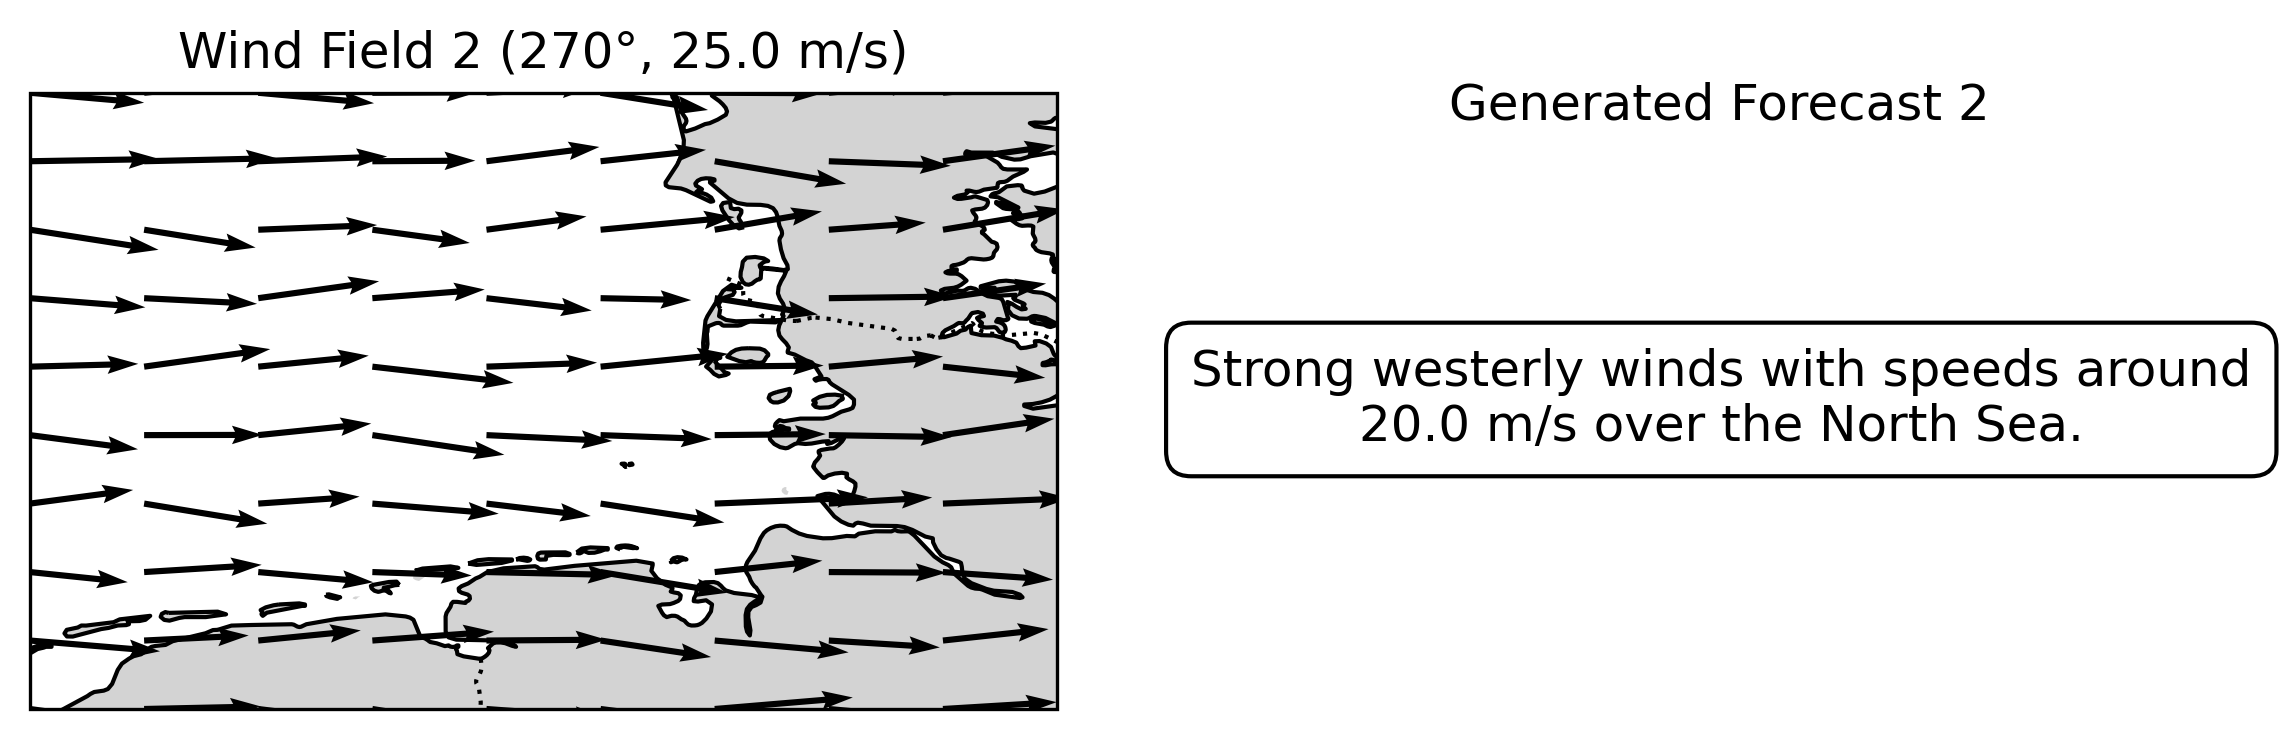
\includegraphics[width=0.45\textwidth]{images/coastal_fcst_01.png} \\
        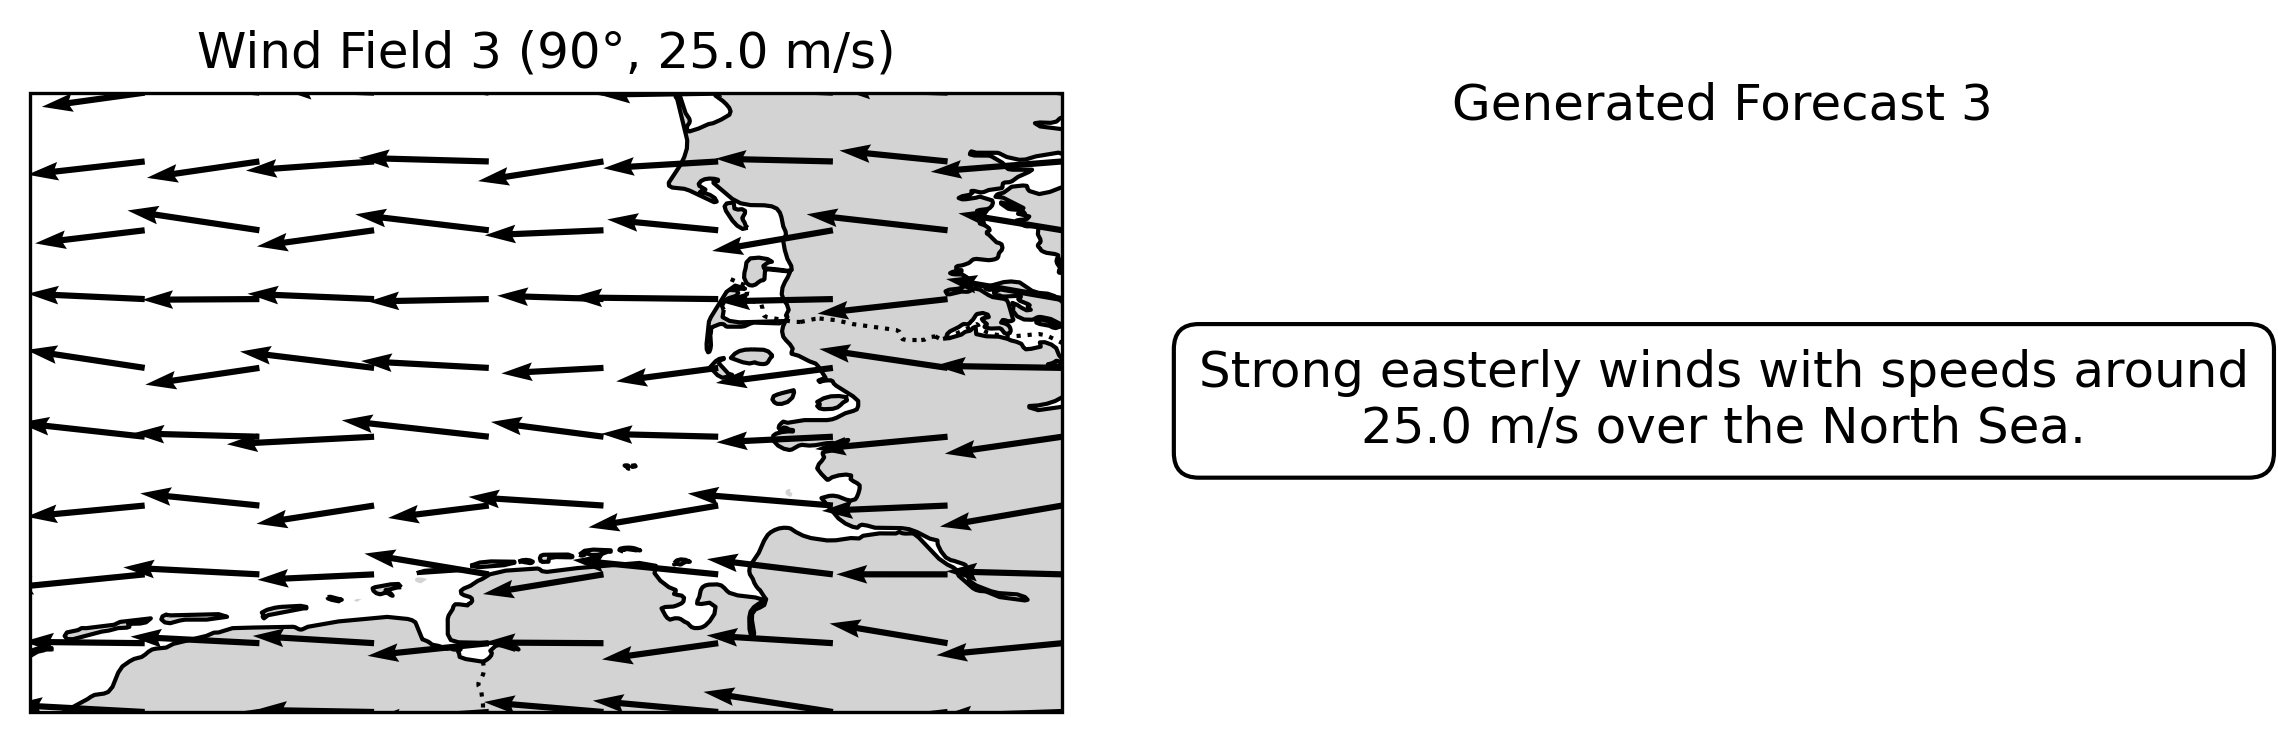
\includegraphics[width=0.45\textwidth]{images/coastal_fcst_02.png} & 
        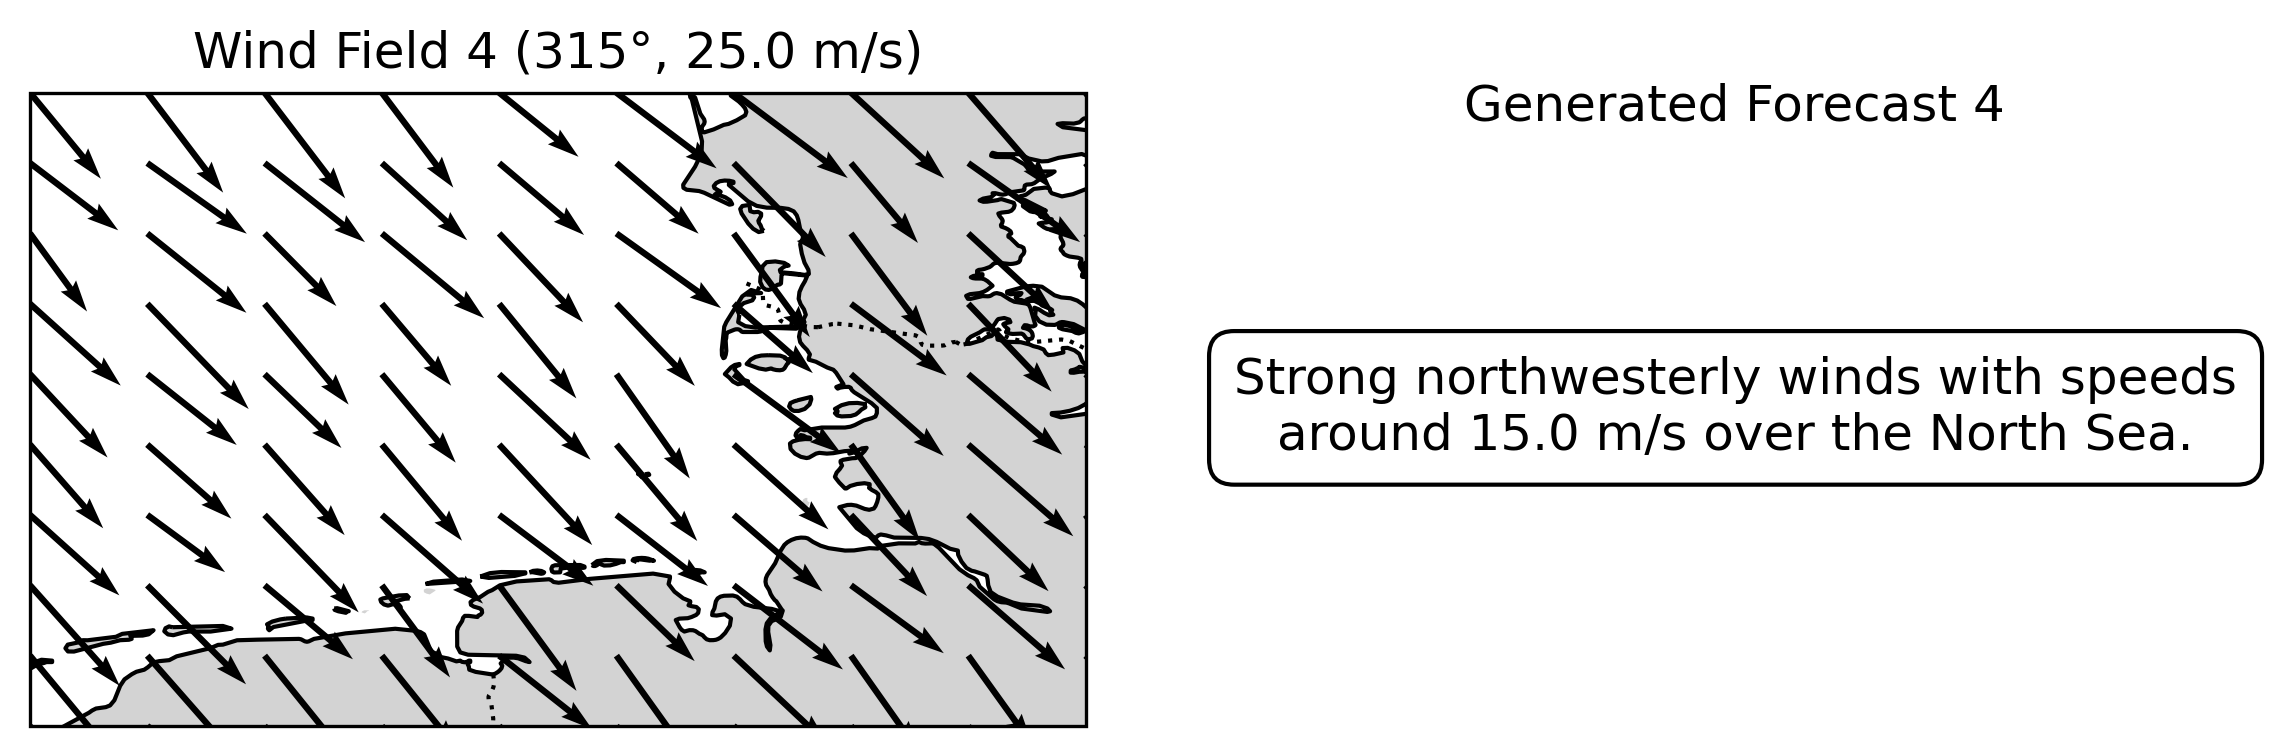
\includegraphics[width=0.45\textwidth]{images/coastal_fcst_03.png} \\
        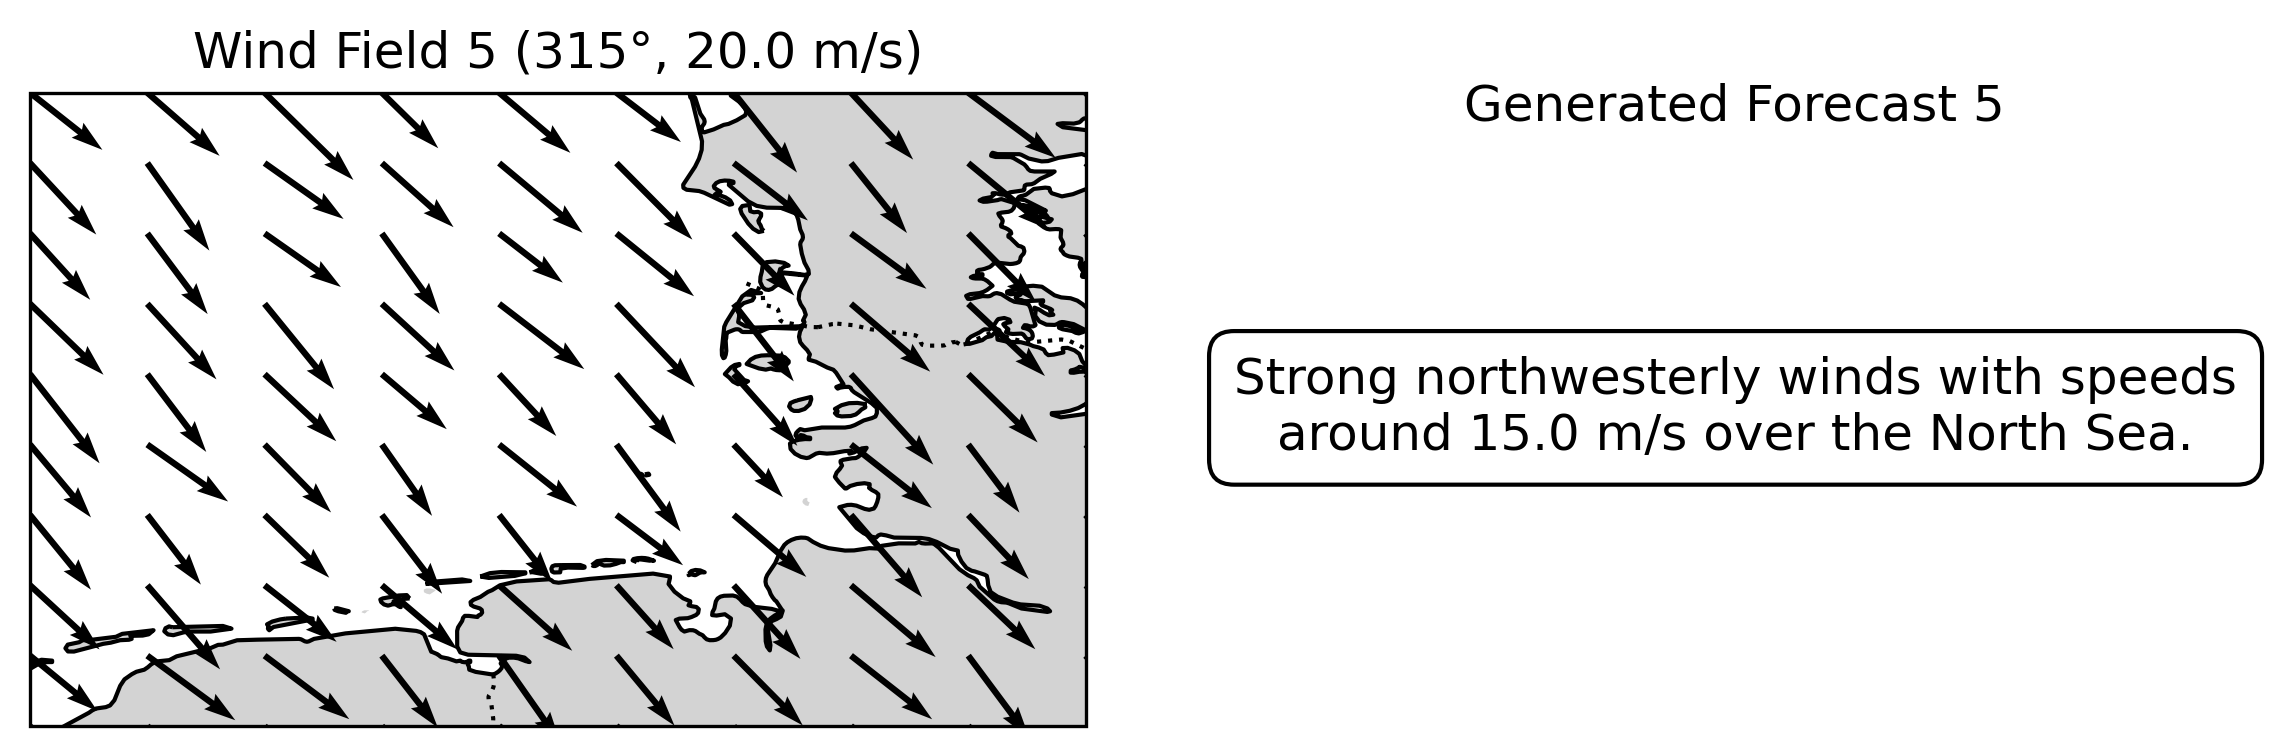
\includegraphics[width=0.45\textwidth]{images/coastal_fcst_04.png} & 
        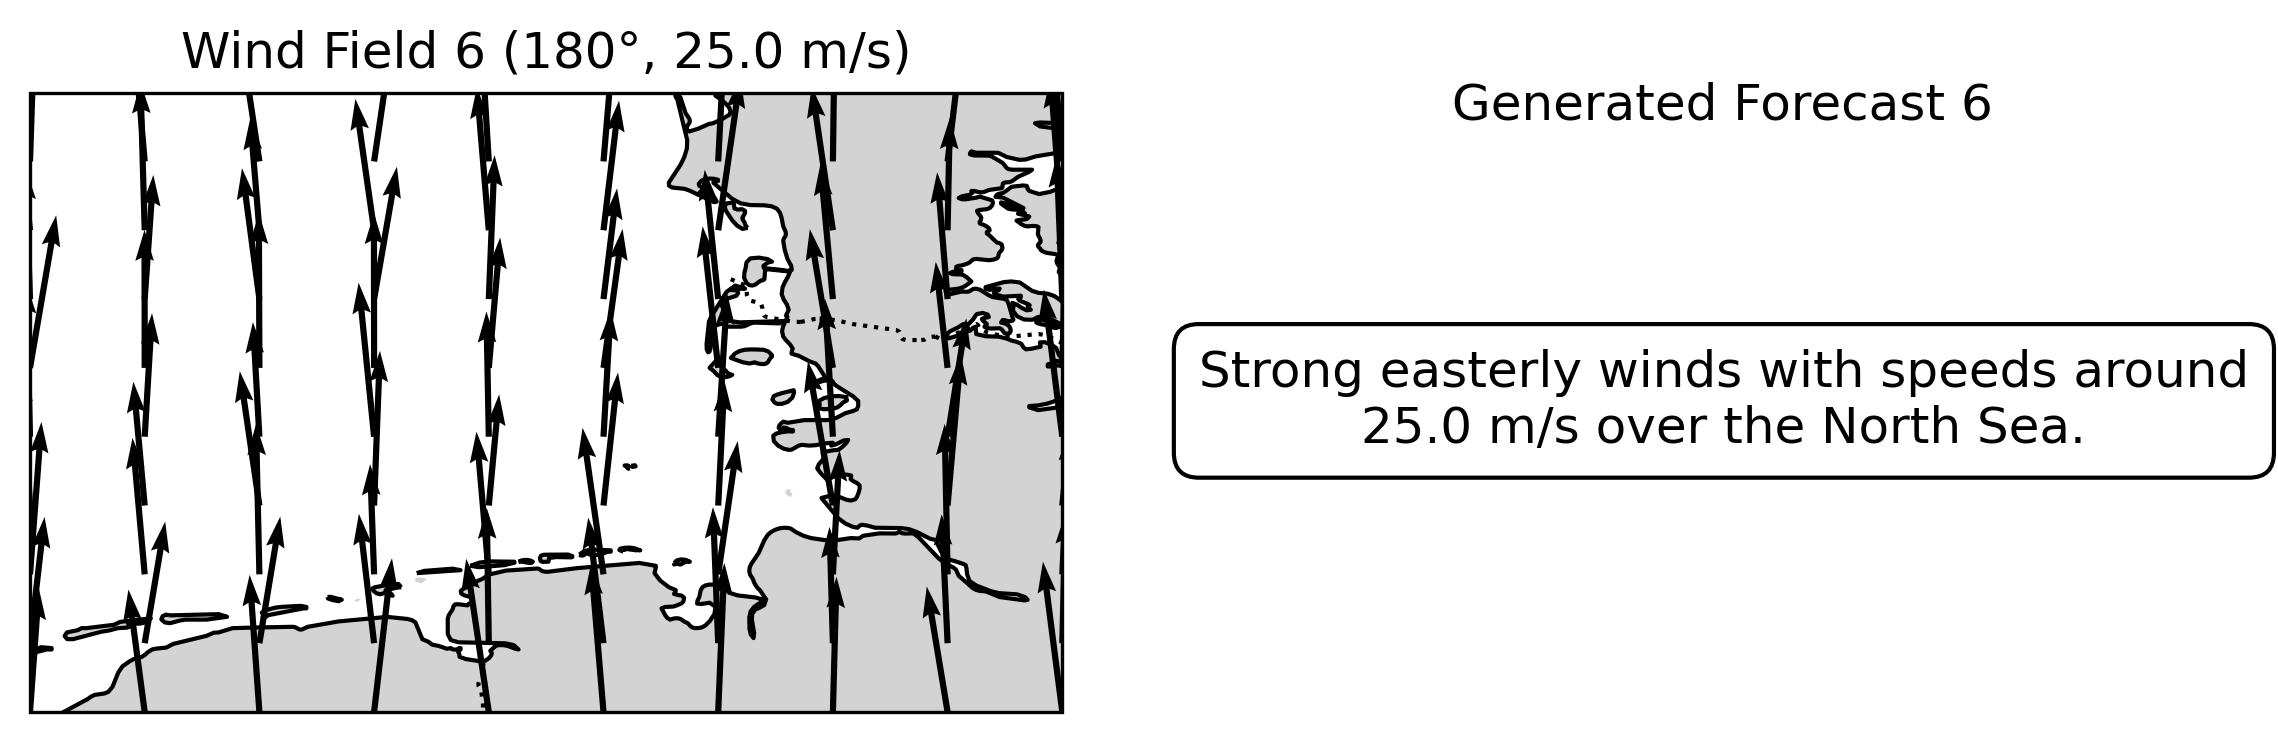
\includegraphics[width=0.45\textwidth]{images/coastal_fcst_05.png} \\
    \end{tabular}
    \caption{Forecast of Coastal Weather at Different Time Steps}
    \label{fig:coastal_forecast}
\end{figure}

{\bf Generating Forecasts}

Once trained, the model can generate textual descriptions from new wind fields:

\begin{codeonly}{Generate Forecasts}
def generate_forecast(model, tokenizer, wind_field):
    U, V = wind_field
    wind_input = f"Wind field: U: {' '.join(map(str, np.round(U.flatten()[:20], 2)))}; V: {' '.join(map(str, np.round(V.flatten()[:20], 2)))}."
    input_ids = tokenizer.encode(wind_input, return_tensors="pt", truncation=True, max_length=512).to(device)
    output = model.generate(input_ids)
    return tokenizer.decode(output[0], skip_special_tokens=True)
\end{codeonly}

%==================================================================================================
%
%==================================================================================================
\section{Radar Data Access and AI Interpretation}

This section documents the steps taken in the Jupyter notebook to access, process, visualize, and interpret radar reflectivity data from the German Weather Service (DWD), using AI-based image analysis via the OpenAI API. The steps are implemented in Python and follow a modular structure.

%==================================================================================================
%
%==================================================================================================
\subsection{1. Downloading the Radar Composite}

Radar composite data in HDF5 format was obtained from the DWD Open Data server. The file was selected from the \texttt{/weather/radar/composite/hx/} directory, which typically contains reflectivity products. The latest file was identified and downloaded automatically.

\begin{codeonly}{python}
import requests
from bs4 import BeautifulSoup
from urllib.parse import urljoin

base_url = "https://opendata.dwd.de/weather/radar/composite/hx/"
response = requests.get(base_url)
soup = BeautifulSoup(response.text, "html.parser")

hd5_files = sorted([
    a.get("href") for a in soup.find_all("a")
    if "composite_hx" in a.get("href", "") and "-hd5" in a.get("href", "")
])

if hd5_files:
    latest_file = hd5_files[-1]
    download_url = urljoin(base_url, latest_file)
    with open("radar.h5", "wb") as f:
        f.write(requests.get(download_url).content)
\end{codeonly}


\begin{figure}[h]
  \centering
  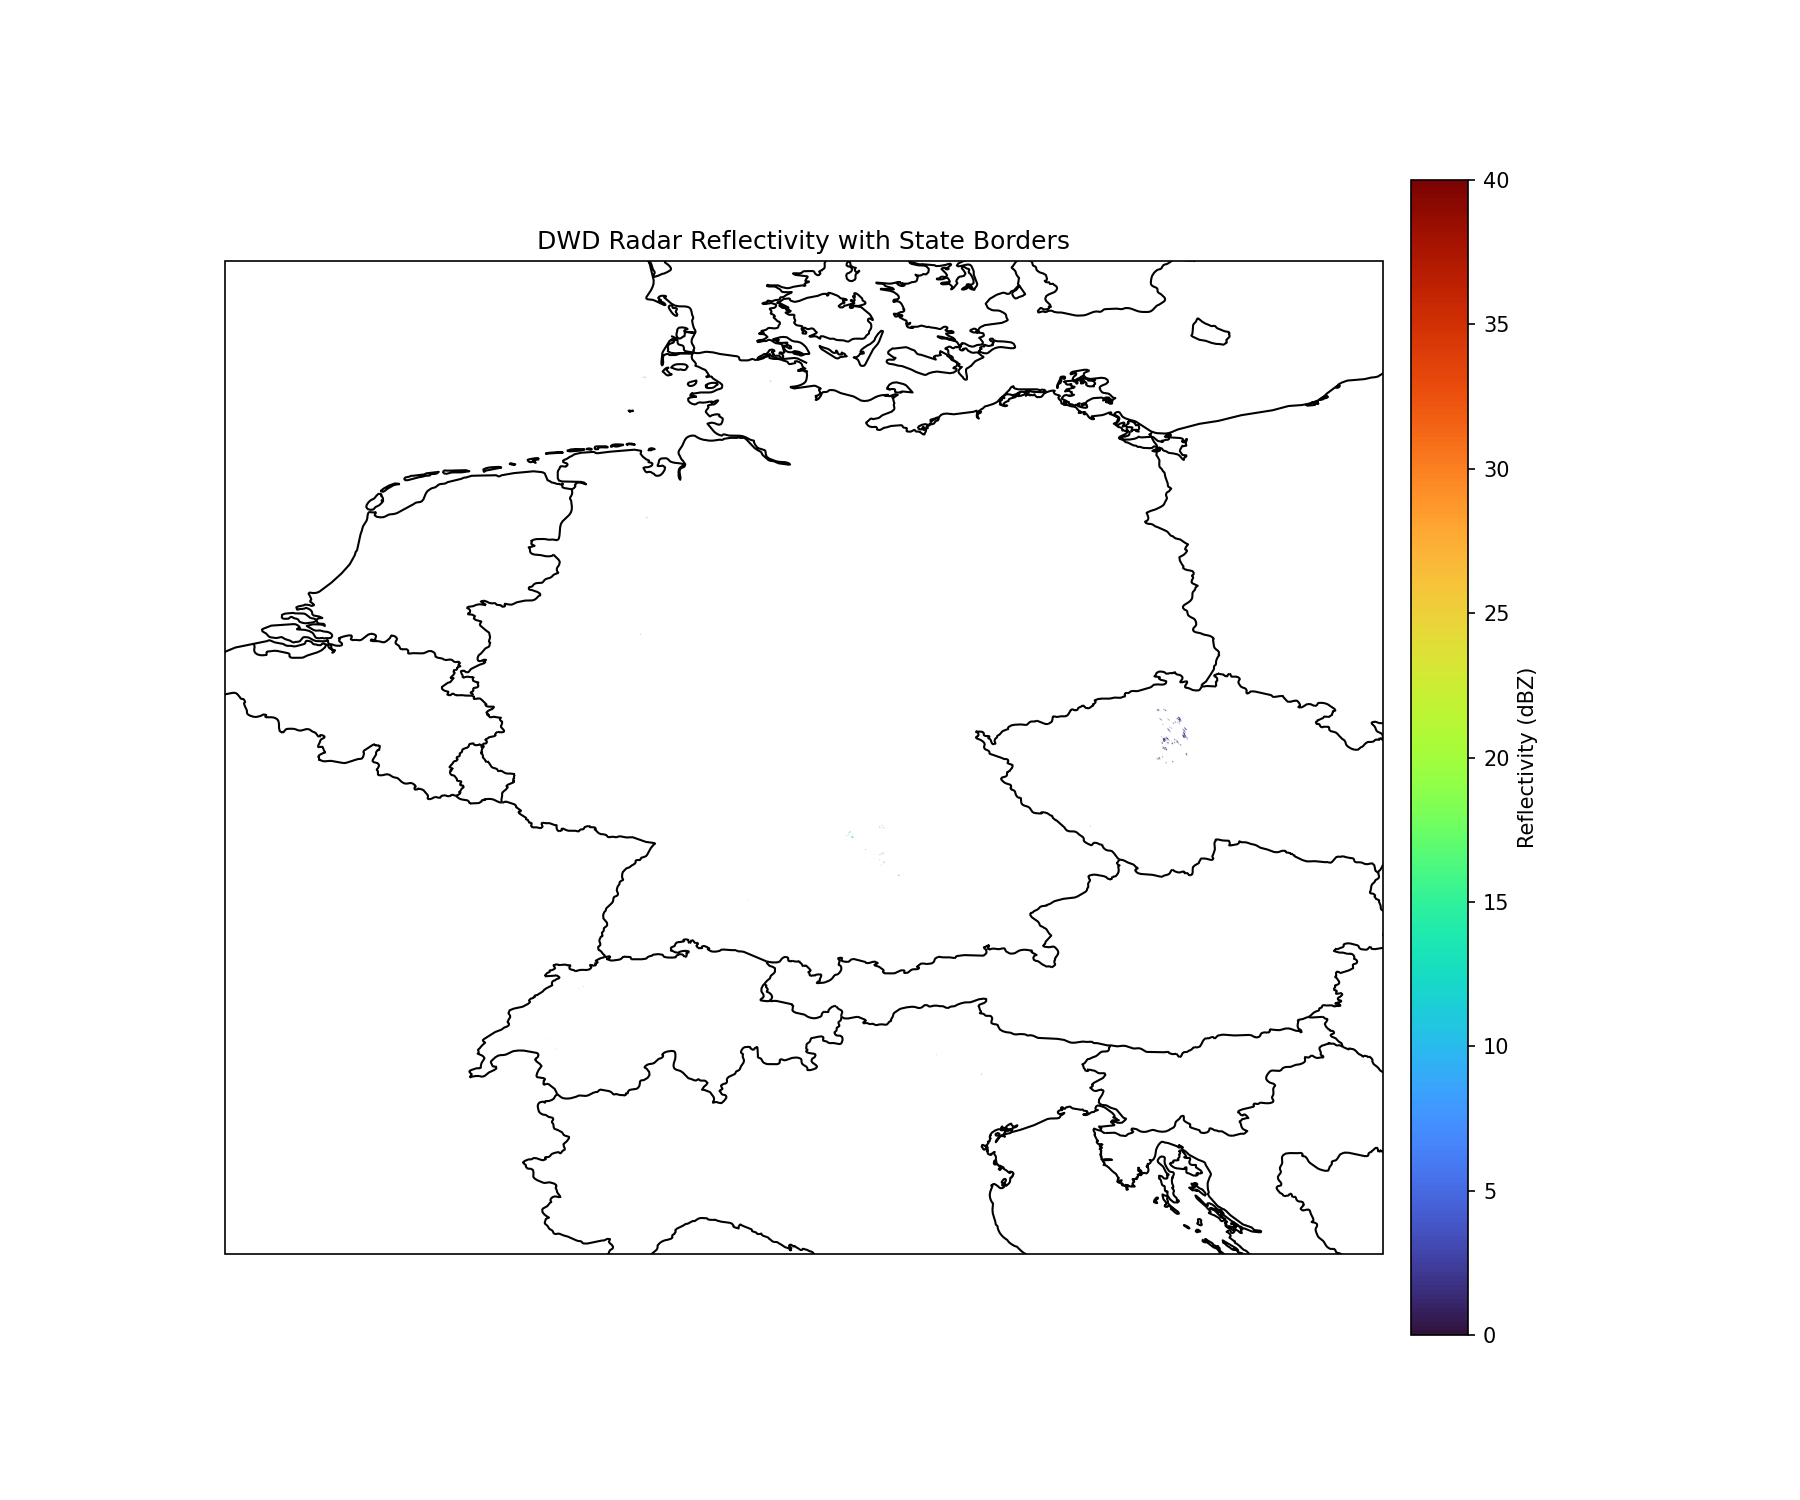
\includegraphics[width=0.9\textwidth]{images/radar_map_germany.png}
  \caption{Decoded radar reflectivity over Germany with state borders. White regions indicate no signal or missing data.}
\end{figure}


%==================================================================================================
%
%==================================================================================================
\subsection{2. Reading and Decoding Reflectivity Data}

The reflectivity field was read from the \texttt{dataset1/data1/data} group in the HDF5 file. The physical reflectivity values (in dBZ) were reconstructed using gain and offset parameters stored in the metadata.

\begin{codeonly}{python}
import h5py
import numpy as np

with h5py.File("radar.h5", "r") as f:
    raw = f["dataset1/data1/data"][:]
    what = f["dataset1/data1/what"]
    gain = what.attrs.get("gain", 1.0)
    offset = what.attrs.get("offset", 0.0)
    reflectivity = raw.astype(np.float32) * gain + offset
    reflectivity[(raw == 0) | (raw == 65535) | (reflectivity < 0)] = np.nan
\end{codeonly}

\subsection{3. Plotting the Radar Composite}

The radar reflectivity is  visualized on a map using Cartopy. The extent was set to cover Germany and surrounding countries. Missing values were shown in white to emphasize actual radar returns.

\begin{codeonly}{python}
import matplotlib.pyplot as plt
import cartopy.crs as ccrs
import cartopy.feature as cfeature
from matplotlib import colormaps

cmap = colormaps.get_cmap("turbo").copy()
cmap.set_bad(color='white')

extent = [3.0, 17.0, 44.0, 56.0]
masked = np.ma.masked_invalid(reflectivity)

plt.figure(figsize=(12, 10))
ax = plt.axes(projection=ccrs.PlateCarree())
ax.set_extent(extent)
im = ax.imshow(masked, extent=extent, cmap=cmap, vmin=0, vmax=40,
               origin='lower', transform=ccrs.PlateCarree())

ax.add_feature(cfeature.BORDERS)
ax.coastlines(resolution='10m')
cbar = plt.colorbar(im, ax=ax)
cbar.set_label("Reflectivity (dBZ)")
plt.title("DWD Radar Reflectivity with State Borders")
plt.savefig("radar_map_germany.png", dpi=150)
plt.show()
\end{codeonly}

%==================================================================================================
%
%==================================================================================================
\subsection{4. Interpretation Using OpenAI GPT-4 Vision}

To generate a natural-language interpretation of the radar image, the processed PNG was base64-encoded and sent to the OpenAI API using the GPT-4-Turbo model with vision capabilities.

\begin{itemize}
  \item The request includes both a text prompt and the radar image.
  \item The result is a textual interpretation of reflectivity patterns, estimated intensity, and structure classification (e.g. stratiform or convective).
\end{itemize}

\begin{codeonly}{python}
from openai import OpenAI
from dotenv import load_dotenv
import base64, os
from IPython.display import Markdown, display

load_dotenv()
client = OpenAI(api_key=os.getenv("OPENAI_API_KEY"))

with open("radar_map_germany.png", "rb") as img:
    encoded = base64.b64encode(img.read()).decode("utf-8")

response = client.chat.completions.create(
    model="gpt-4-turbo",
    messages=[
        {"role": "user", "content": [
            {"type": "text", "text": "Interpret this radar reflectivity image from Germany. Describe precipitation areas, intensity, and structure."},
            {"type": "image_url", "image_url": {
                "url": f"data:image/png;base64,{encoded}"}
            }
        ]}
    ],
    max_tokens=800,
)

interpretation = response.choices[0].message.content
display(Markdown(interpretation))
\end{codeonly}

Here is the outcome of the image interpretations, which OpenAI provides. 

\begin{lstlisting}[style=mdstyle]
This image of radar reflectivity from Germany depicts various levels of precipitation intensity across different regions, as indicated by the color scale on the right. The color scale ranges from 0 dBZ, representing no precipitation, to 40 dBZ, indicating heavy precipitation.

In this image:

Northwestern Germany: There appears to be no significant precipitation as the colors are in the lower range of the scale (0-5 dBZ), which is indicative of clear or very light precipitation conditions.

Northeastern Germany: Similar to the northwest, this region also shows minimal reflectivity values, indicating little to no precipitation.

Central and Southern Germany: These areas also display minimal radar reflectivity with dBZ values primarily in the range of 0-5 dBZ. There seem to be no significant precipitation events occurring in these regions at the time this image was captured.

Western and Southwestern Germany: These regions are predominantly clear, with a few areas perhaps having very light precipitation as indicated by slightly higher, but still minimal dBZ values.

There are no distinct areas of high dBZ values (e.g., >20 dBZ) that would suggest moderate to heavy rainfall or convective activity (such as thunderstorms) anywhere on the map. Therefore, the image overall does not show any signs of significant convective structures such as thunderstorm cells, which would typically be indicated by localized, high-intensity dBZ readings.

All in all, the weather across Germany during the period represented by this reflectivity image seems to be largely calm and free of significant precipitation events, with only scattered, very light precipitation or clear conditions throughout. The absence of any high dBZ values indicates an absence of strong convective activities like thunderstorms, which are typically characterized by sudden, intense rainfall indicated by higher dBZ values.
\end{lstlisting}

We note that the interpretation will be billed by standard platforms as shown in the following figure. 

\begin{figure}[ht]
  \centering
  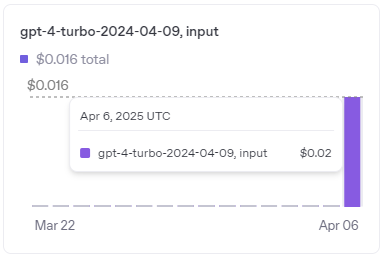
\includegraphics[width=0.49\textwidth]{images/billing_gpt_4_turbo_in2.png}
  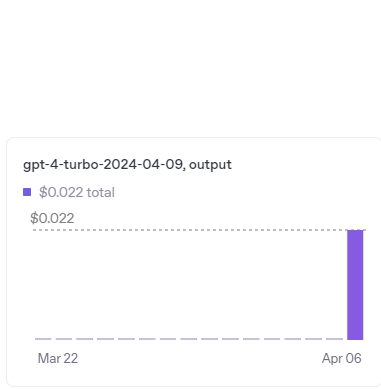
\includegraphics[width=0.49\textwidth]{images/billing_gpt_4_turbo_out2.png}
  \caption{Input and Output for image interpretation will cost, here about 2-3 cent per image (in and out summed).}
\end{figure}

%==================================================================================================
%
%==================================================================================================
\section{Cloud Top Height as a Multimodal AI Application}

Cloud Top Height (CTH) is a satellite-derived parameter that estimates the altitude of the upper boundary of cloud systems, typically expressed in meters above sea level. It is primarily derived from thermal infrared satellite observations (e.g., from Meteosat SEVIRI), which allow cloud top temperature to be estimated and then converted to height using vertical atmospheric profiles.

High CTH values are generally associated with deep convective systems such as cumulonimbus clouds, while low CTH values are often indicative of stratiform or shallow cloud layers. As such, CTH provides valuable insight into atmospheric structure and storm development, especially in the absence of direct vertical sounding data.

In the context of multimodal AI, CTH maps are well suited for image-text applications, where visual patterns are interpreted in conjunction with meteorological knowledge. Below, we outline several possible use cases for applying multimodal models (e.g., GPT-4 with Vision or Gemini) to CTH data.

%==================================================================================================
%
%==================================================================================================
\subsection{Multimodal Use Cases for Cloud Top Height Interpretation}

\begin{itemize}
    \item \textbf{CTH Map Interpretation} \\
    Given a single satellite-derived CTH image, a multimodal model can identify regions of high cloud tops (e.g., >10~km), associate them with potential deep convection, and distinguish between different cloud layers. This is useful for nowcasting and synoptic analysis.

    \item \textbf{CTH and Radar Reflectivity Comparison} \\
    A side-by-side analysis of CTH and radar reflectivity fields enables the model to assess where tall clouds are associated with precipitation. This helps in identifying convective cores or in evaluating false alarms, such as high cloud tops without significant rainfall.

    \item \textbf{CTH Overlay with Numerical Weather Prediction (NWP)} \\
    By comparing observed CTH fields with model-predicted convective zones, the AI can evaluate the accuracy of model forecasts, detect missed storms, or highlight overestimates of vertical development. This can support model diagnostics and validation.

    \item \textbf{CTH Threshold-Based Alerting} \\
    AI systems can be tasked with scanning a CTH image and identifying areas exceeding certain height thresholds (e.g., 10,000~m). These regions may be relevant for aviation warnings, thunderstorm alerts, or convective risk assessments.

    \item \textbf{Time-Series or Animation Analysis} \\
    Using a sequence of CTH images, a multimodal model could track the temporal evolution of convective systems. It can describe cloud growth, merging, or dissipation — similar to what a human forecaster might do when watching satellite loops.

    \item \textbf{Natural Language Bulletins from CTH Maps} \\
    The model can automatically generate synoptic summaries or weather briefings based solely on the CTH structure, using meteorological language. This supports automation in forecast generation and situational awareness.

\end{itemize}

These examples demonstrate the broad potential of combining satellite-derived cloud structure with large multimodal models to extract high-level meteorological insights in a human-readable form.


%==================================================================================================
%
%==================================================================================================
\subsection{CTH Map Interpretation}

\begin{figure}[h]
  \centering
  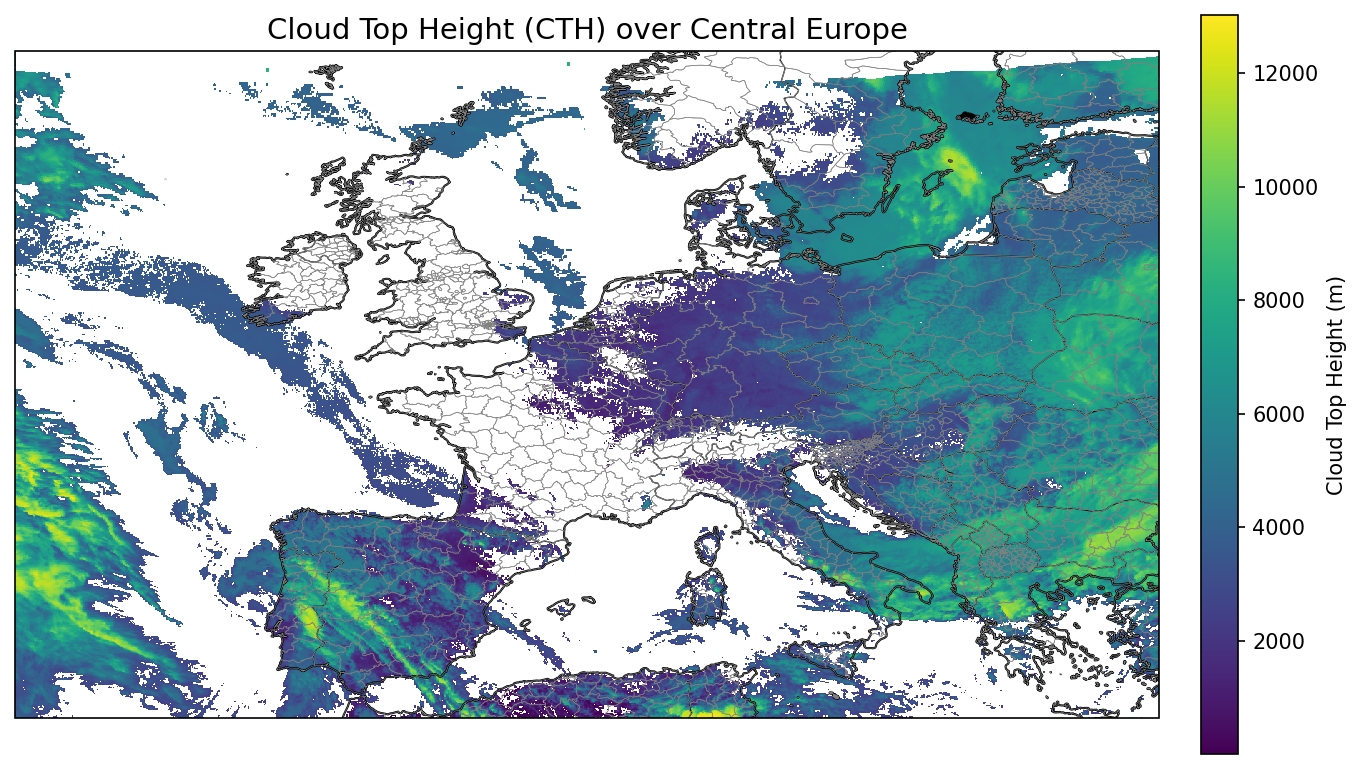
\includegraphics[width=0.9\textwidth]{images/cth_map.png}
  \caption{Cloud Top Height (CTH) over Central Europe derived from satellite data. Higher cloud tops (green/yellow) are indicative of deep convection; lower tops (purple) represent stratiform or less active cloud fields.}
\end{figure}

To interpret the satellite-derived CTH image, the notebook performs the following steps:

\paragraph{1. Download the Latest CTH File}

We start by accessing the latest CTH file from the DWD Open Data server.

\begin{codeonly}{python}
import requests
from bs4 import BeautifulSoup
from urllib.parse import urljoin

base_url = "https://opendata.dwd.de/weather/satellite/clouds/CTH/"
response = requests.get(base_url)
soup = BeautifulSoup(response.text, "html.parser")

cth_files = sorted([
    link.get("href") for link in soup.find_all("a")
    if link.get("href", "").endswith(".nc.bz2")
])

latest_file = cth_files[-1]
download_url = urljoin(base_url, latest_file)

with open("cth_latest.nc.bz2", "wb") as f:
    f.write(requests.get(download_url).content)
\end{codeonly}

\paragraph{2. Decompress and Read the Data}

The `.bz2` archive is unpacked, and the cloud top height data is read from the NetCDF file.

\begin{codeonly}{python}
import bz2
import netCDF4 as nc

with bz2.BZ2File("cth_latest.nc.bz2") as bz2file:
    with open("cth_latest.nc", "wb") as ncfile:
        ncfile.write(bz2file.read())

ds = nc.Dataset("cth_latest.nc")
cth = ds.variables["CTH"][0, :, :]
lat = ds.variables["lat"][:]
lon = ds.variables["lon"][:]
\end{codeonly}

\paragraph{3. Visualize the CTH Field}

A simple pseudocolor map is created using Matplotlib, where high cloud tops are shown in brighter colors.

\begin{codeonly}{python}
import numpy as np
import matplotlib.pyplot as plt

cth = np.ma.masked_where(cth <= 0, cth)

plt.figure(figsize=(10, 8))
plt.pcolormesh(lon, lat, cth, cmap="viridis", shading="auto")
plt.colorbar(label="Cloud Top Height (m)")
plt.title("Cloud Top Height (latest observation)")
plt.xlabel("Longitude")
plt.ylabel("Latitude")
plt.grid(True)
plt.savefig("cth_map.png", dpi=150)
plt.show()
\end{codeonly}

\paragraph{4. AI-Based Interpretation with OpenAI Vision.}

The image is encoded and sent to OpenAI's multimodal model through its platform API for meteorological interpretation.

\begin{codeonlysmall}{python}
from openai import OpenAI
from dotenv import load_dotenv
import os
import base64
from IPython.display import Markdown, display

load_dotenv()
client = OpenAI(api_key=os.getenv("OPENAI_API_KEY"))

with open("cth_map.png", "rb") as image_file:
    base64_image = base64.b64encode(image_file.read()).decode("utf-8")

response = client.chat.completions.create(
    model="gpt-4-turbo",
    messages=[
        {
            "role": "user",
            "content": [
                {
                    "type": "text",
                    "text": (
                     "This is a satellite-derived Cloud Top Height (CTH) image over Europe."
                        "Please interpret the structure shown in the image: \n"
                        "- Identify regions of high or low cloud tops.\n"
                        "- Estimate where deep convection may be present.\n"
                        "- Describe what synoptic or convective features are visible.\n"
                        "- Provide a summary of the possible weather situation."
                    )
                },
                {
                    "type": "image_url",
                    "image_url": {
                        "url": f"data:image/png;base64,{base64_image}"
                    }
                }
            ]
        }
    ],
    max_tokens=800,
)

interpretation = response.choices[0].message.content
display(Markdown(interpretation))
\end{codeonlysmall}


Here is the outcome of the image interpretations, which our script based on the OpenAI API provides. 

\begin{lstlisting}[style=mdstyle]
Identification of Regions of High and Low Cloud Tops:

High Cloud Tops:
Central Northern Europe, especially in the yellow-colored area over central Sweden and parts of Norway, displays very high cloud tops that exceed 10,000 meters. Some high cloud tops are also noticeable over the sea directly west of the Iberian peninsula.

Low Cloud Tops:
Major parts of the European mainland have lower cloud tops, particularly noticeable in France, Germany, and extending eastward across Poland into parts of Russia (indicated by purple to blue colors), where cloud tops range from 2000 to 6000 meters.

Potential Areas of Deep Convection:
The high cloud tops observed particularly in central parts of Scandinavia (central Sweden and nearby areas) are potential indicators of deep convective activity. Typically, cloud tops reaching or exceeding heights around 10,000 meters suggest the presence of cumulonimbus clouds, which are associated with heavy rainfall, thunderstorms, and potential severe weather events.

Visible Synoptic or Convective Features:
An intense convective system appears to be over Central Scandinavia, supported by the very high cloud tops as indicated by the yellow coloration. This system may suggest the development or presence of a strong weather front, potentially a cold front given its structure and scale.

Widespread lower cloud tops across much of Western and Eastern Europe might be associated with stable weather patterns or widespread stratiform clouds usually seen with settled conditions or behind a front.

Possible Summary of the Weather Situation:
The presence of high, deep convective cloud tops over Central Scandinavia suggests ongoing or developing strong weather activities, likely associated with significant rainfall, thunderstorms, or possibly snow if temperatures are low enough.

In contrast, much of the rest of the Central European region, characterized by lower cloud tops, might be experiencing more stable and milder weather. This could manifest as cloudy but largely dry conditions, potentially following the passage of a weather front.

The contrasting cloud top heights from the west to the east may indicate a strong weather gradient, potentially impacting weather conditions rapidly over short distances in the region.

In conclusion, the satellite-derived CTH image suggests significant weather activity, particularly over Scandinavia, with potential impacts including precipitation and more pronounced weather events, while a quieter weather regime may prevail over large parts of Western and Central Europe.
\end{lstlisting}
